\section{Конструкторский раздел}

\subsection{Описание сущностей проектируемой базы данных}

В базе данных будет существовать 5 сущностей и 6 таблиц, одна из которых является развязочной. 
\begin{figure}[hbtp]
	\centering
	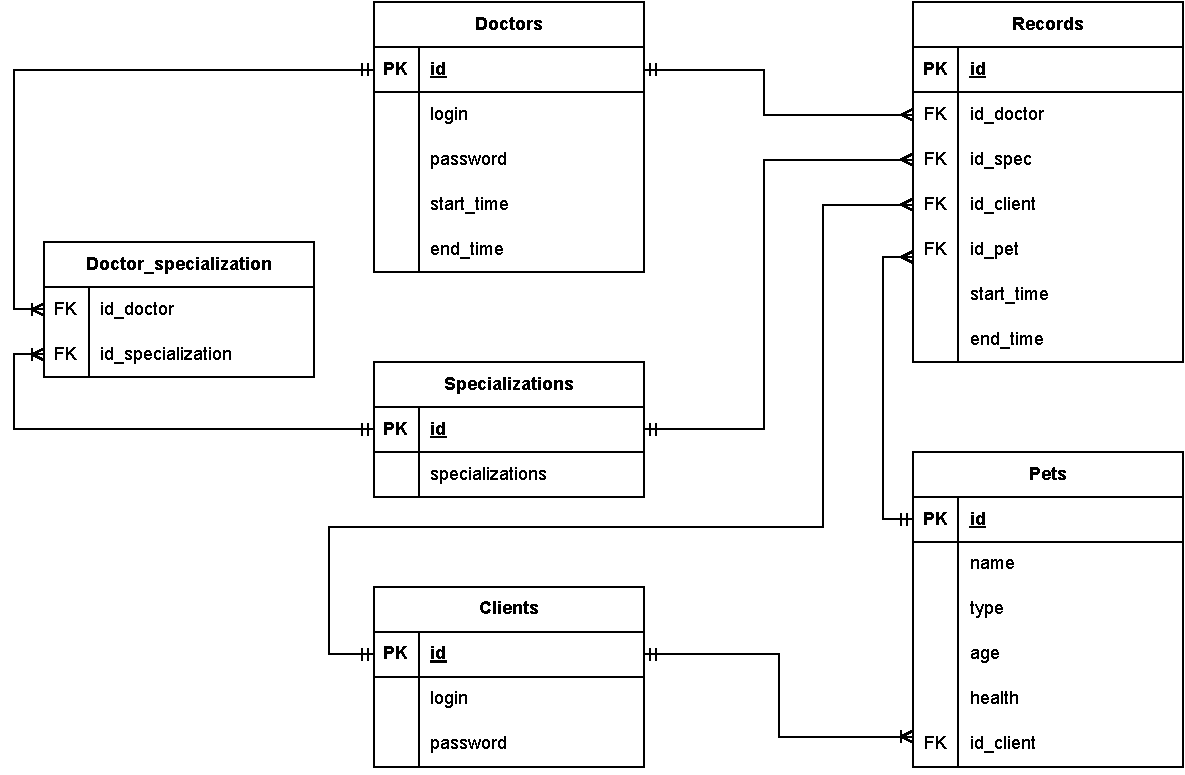
\includegraphics[width=150mm]{image/bd.pdf}
	\caption{Диаграмма проектируемой базы данных}
	\label{img:idef}
\end{figure}

Необходимы следующие таблицы.
\begin{enumerate}[label=\arabic*)]
	\item Таблица c работниками клиники, то есть докторами (Doctors).
	\item Таблица для специализаций работников клиники (Specializations).
	\item Развязочная таблица для работников и их специализаций.
	\item Таблица c клиентами клиники (Clients).
	\item Таблица c питомцами клиники (Pets).
	\item Таблица c записями на прием (Records).
\end{enumerate}

В таблице \ref{tab:doctors}  описаны поля таблицы Doctors. В таблице \ref{tab:specializations} описаны поля таблицы Specializations. В таблице \ref{tab:DC} описаны поля таблицы связки для Doctors и Specializations. Сейчас таблица Specializations содержит только идентификатор и название специализации (например, ветеринар-фельдшер), поэтому можно было бы обойтись без отдельной таблицы для специализаций и следовательно без таблицы-связки. Но она реализована для легкого расширения функционала, к примеру, можно добавить стаж или уровень владения конкретной специальностью.

\begin{table}[hbtp]
	\begin{center}
			\captionsetup{justification=raggedright, singlelinecheck=false}
			\caption{\label{tab:doctors}Поля таблицы Doctors}
		\begin{tabular}{|l|l|l|l|l|l|}
			\hline {Поле} & {Тип данных} & {Описание}  \\ \hline
			id  & int & Идентификатор работника   \\ \hline
			login & text & Идентификатор работника для входа в систему \\ \hline
			password & text & Пароль работника для входа в систему  \\ \hline
			shedule & text & Расписание, то есть часы приема\\ \hline
		\end{tabular}
	\end{center}
\end{table}

\begin{table}[hbtp]
	\begin{center}
		\captionsetup{justification=raggedright, singlelinecheck=false}
		\caption{\label{tab:specializations}Поля таблицы Specializations}
		\begin{tabular}{|l|l|l|l|l|l|}
			\hline {Поле} & {Тип данных} & {Описание}  \\ \hline
			id  & int & Идентификатор специализации \\ \hline
			specialization & text & Название специализации\\ \hline
		\end{tabular}
	\end{center}
\end{table}

\begin{table}[hbtp]
	\begin{center}
		\captionsetup{justification=raggedright, singlelinecheck=false}
		\caption{\label{tab:DC}Поля развязочной таблицы Doctors-Specializations}
		\begin{tabular}{|l|l|l|l|l|l|}
			\hline {Поле} & {Тип данных} & {Описание}  \\ \hline
			id\_doctor  & int & Идентификатор доктора \\ \hline
			id\_specialization & int & Идентификатор специализации \\ \hline
		\end{tabular}
	\end{center}
\end{table}

В таблице \ref{tab:clients}  описаны поля таблицы Clients. Хоть клиенты и работники имеют 3 одинаковых поля, но они разнесены по разным таблицам, ибо у них разные роли в бизнес-процессах. Разделение позволяет лучше структурировать информацию и дополнительные связи с другими сущностями. В таблице \ref{tab:pets}  описаны поля таблицы Pets. В данном проекте у питомца может быть только один владелец, но у владельца может быть много питомцев. Поэтому информация о связи питомец-владелец реализуется с помощью таблицы Pets, где содержится идентификатор хозяина. 

\begin{table}[hbtp]
	\begin{center}
		\captionsetup{justification=raggedright, singlelinecheck=false}
		\caption{\label{tab:clients}Поля таблицы Clients}
		
		\begin{tabular}{|l|l|l|l|l|l|}
			\hline {Поле} & {Тип данных} & {Описание}  \\ \hline
		id  & int & Идентификатор клиента   \\ \hline
		login & text & Идентификатор клиента для входа в систему \\ \hline
		password & text & Пароль клиента для входа в систему  \\ \hline
		\end{tabular}
	\end{center}
\end{table}

\begin{table}[hbtp]
	\begin{center}
			\captionsetup{justification=raggedright, singlelinecheck=false}
			\caption{\label{tab:pets}Поля таблицы Pets}
		\begin{tabular}{|l|l|l|l|l|l|}
			\hline {Поле} & {Тип данных} & {Описание}  \\ \hline
			id  & int & Идентификатор питомца   \\ \hline
			name & text & Кличка питомца \\ \hline
			type & text & Вид, порода питомца  \\ \hline
			age & int & Возраст питомца \\ \hline
			health & int & Уровень здоровья питомца  \\ \hline
			id\_client & int & Идентификатор хозяина  \\ \hline
		\end{tabular}
	\end{center}
\end{table}

В таблице \ref{tab:records}  описаны поля таблицы Records, которая хранит записи на прием. Можно заметить, что таблица не хранит идентификатор хозяина, потому что его можно получить из информации о питомце. 

\begin{table}[hbtp]
		\captionsetup{justification=raggedright, singlelinecheck=false}
		\caption{\label{tab:records}Поля таблицы Records}
	\begin{center}
		\begin{tabular}{|l|l|l|l|l|l|}
			\hline {Поле} & {Тип} & {Описание}  \\ \hline
			id  & int & Идентификатор приема   \\ \hline
			id\_doctor & int & Идентификатор доктора  \\ \hline
			id\_pet & int & Идентификатор питомца   \\ \hline
			date\_record & date & Дата приема \\ \hline
			time\_start & time & Время начала приема  \\ \hline
		\end{tabular}
	\end{center}
\end{table}

\pagebreak

\subsection{Ролевая модель}
Исходя из функциональности, предъявляемой к приложению и представленной на рисунке \ref{img:use-case} можно выделить следующие роли:
\begin{enumerate}[label=\arabic*)]
	\item Гость. Имеет права только на просмотр таблиц сотрудников и их специализаций, это считается просмотром предоставляемых услуг.
	\item Клиент. Имеет права на просмотр и изменение записей, связанных с ним и его питомцами в таблицах Clients, Pets, Records. Как и гость может смотреть предоставляемые услуги.
	\item Работник. Имеет права на просмотр и изменение всех таблиц, кроме таблицы Clients. В таблице Сlients не может видеть и изменять пароль клиента, то есть поле password.  
\end{enumerate}

\subsection{Триггеры базы данных}

Для обеспечения актуальной информации в базе данных ветеринарной клиники выделены триггеры, реализующие следующую логику.
\begin{enumerate}[label=\arabic*)]
	\item При изменении расписания сотрудника, все записи на прием, которые не попадают в новый график работы, удаляются. 
	\item При удалении питомца также удаляются все его записи на прием, который еще не были совершены.
\end{enumerate}

\subsection{Транзакции базы данных}
Для поддержания непротиворечивости базы данных следующие операции выделены в транзакции.

\begin{enumerate}[label=\arabic*)]
	\item Добавление, изменение или удаление любой информации о клиентах, сотрудниках или питомцах. 
	\item Операции с записью на прием. Это особенно важно, так как поможет избежать ошибок в расписании работников клиники.
	\item Результат работы триггеров. 
\end{enumerate}


\subsection*{Вывод}
В данном разделе были описаны сущности и ролевая модель проектируемой базы данных. Также были спроектированы триггеры и транзакции.